\documentclass{article}
\usepackage[utf8]{inputenc}
\usepackage{authblk}
\usepackage{setspace}
\usepackage[margin=1.25in]{geometry}
\usepackage{graphicx}
\usepackage{xcolor}
\usepackage{float}
\graphicspath{ {./figures/} }
\usepackage{amsmath,amssymb,amsfonts}
\usepackage{booktabs}
\usepackage{natbib}
\usepackage{hyperref}
\hypersetup{colorlinks=true, linkcolor=blue, citecolor=blue, urlcolor=blue}

\title{\textbf{Gradient Boosting and Next-Day Equity Direction: A Walk-Forward Test with Cross-Asset Features}}
\author[1]{SIQuant Research}
\affil[1]{Hypothesis $\times$ Quant}
\date{\today}
\onehalfspacing

\begin{document}
\maketitle

\begin{abstract}
\noindent \textbf{Hypothesis:} $H_0$: the out-of-sample ROC AUC of the gradient-boosting classifier for the next-day S\&P 500 direction equals 0.5; $H_1$: it is larger \\
\textbf{Data:} 1,963 out-of-sample sessions, 2019-01-02 to 2026-10-22, 12 cross-asset features published by the close \\
\textbf{Method:} Yearly walk-forward folds with a 5-day embargo, fixed hyper-parameters, logistic-regression baseline, 5,000-draw label-permutation test \\
\textbf{Results:} GBM AUC 0.5068 (permutation $p=0.3081$), logistic AUC 0.4894; accuracy 53.1\% versus 54.7\% for always predicting the majority class. \\
\textbf{Research decision:} \colorbox[rgb]{0.75,0.15,0.15}{\textcolor{white}{\textbf{\,REJECTED\,}}}
\end{abstract}

\section{Design}
The target is the sign of the next-day S\&P 500 return, a task for which return predictability is known to be weak \citep{gu2020empirical}. Features use only information published by the close of day $t$; each yearly fold trains on earlier years with an embargo of five sessions before the test year. Hyper-parameters are fixed before the evaluation, and nothing is tuned on out-of-sample data.

\section{Results}
A long-short rule that follows the predicted sign has an annualised Sharpe ratio of 0.47 before costs (descriptive only).

\begin{figure}[H]
\centering
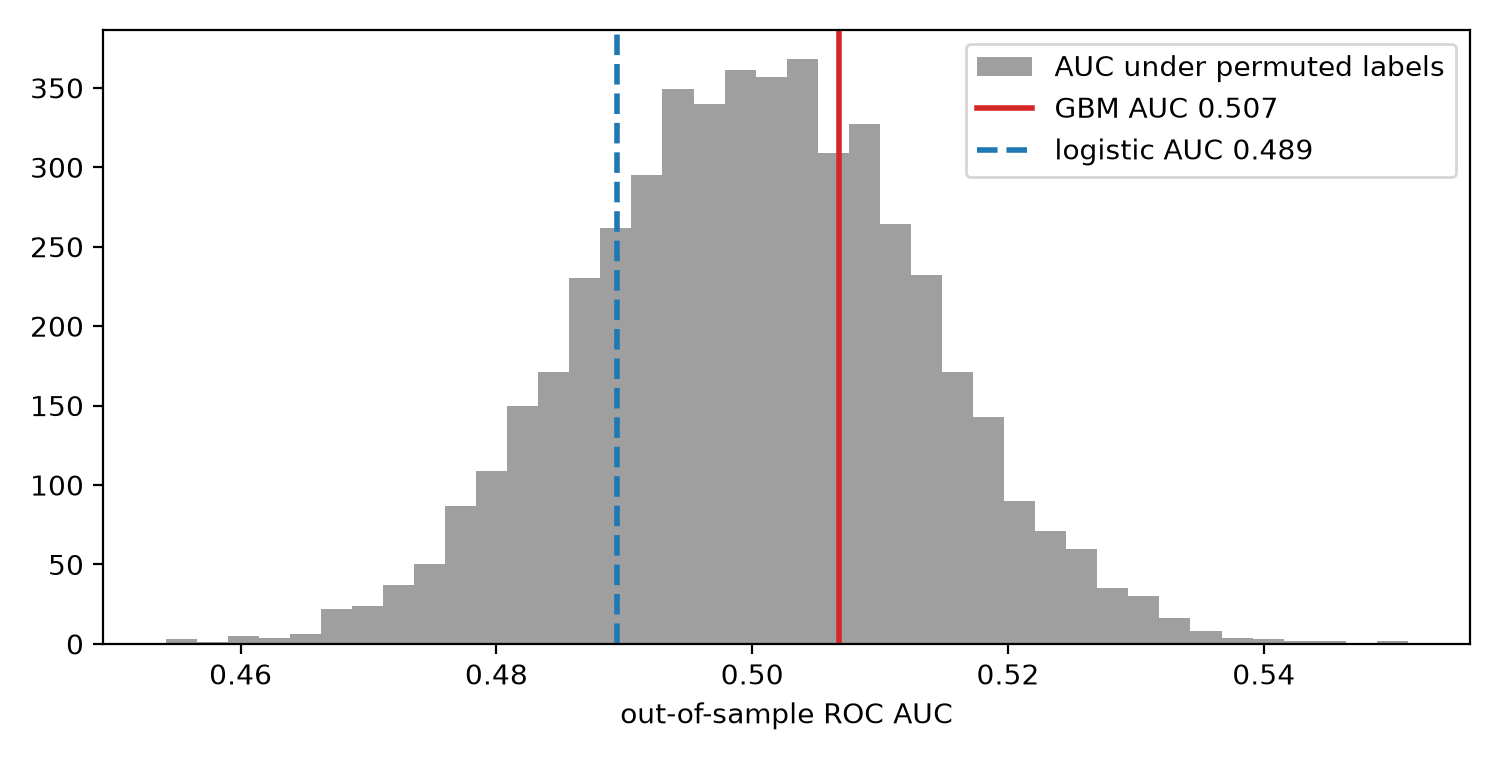
\includegraphics[width=0.8\textwidth]{fig1_auc_permutation.png}
\caption{Out-of-sample AUC against the permutation distribution.}
\end{figure}

\section{Limitations}
Permuting labels treats daily directions as exchangeable, which is a good approximation for daily index returns but ignores volatility clustering. An AUC above 0.5 does not imply a tradable edge after costs. All features come from Yahoo Finance and FRED closes that are not perfectly synchronous.


\bibliographystyle{plainnat}
\bibliography{references}

\end{document}
